\documentclass[12pt]{article}

% =========================
% preamble.tex (PROJECT POSTER DESIGN SYSTEM)
% =========================

% Language + math
\usepackage[english]{babel}
\usepackage{latexsym,amssymb,amsmath,amsfonts}
\usepackage{bm}

% Layout + multi-columns
\usepackage{geometry}
\usepackage{multicol}
\usepackage{paralist}
\usepackage{enumitem}

% Graphics
\usepackage[pdftex]{graphicx}
\DeclareGraphicsExtensions{.jpg,.pdf,.pdftex,.png}
\graphicspath{{./figures/}}

% Links
\usepackage[colorlinks=true,linkcolor=PosterBlue,urlcolor=black,citecolor=PosterBlue]{hyperref}

% Tables
\usepackage{booktabs}
\usepackage{tabularx}
\usepackage{array}
\newcolumntype{C}{>{\centering\arraybackslash}X}

% TikZ / PGFplots (optional diagrams)
\usepackage{tikz}
\usepackage{pgfplots}
\usetikzlibrary{shapes,calc,backgrounds,fit,patterns,shadings,shadows}
\pgfplotsset{compat=1.18}

% Icons
\usepackage{pifont}
\usepackage{fontawesome}

% Boxes
\usepackage{tcolorbox}
\tcbuselibrary{skins,breakable}

% Caption
\usepackage{caption}
\usepackage{subfig}
\usepackage{float}
\usepackage{wrapfig}

% -------------------------------------------------
% POSTER PAGE GEOMETRY (A0-ish: 420x594mm)
% -------------------------------------------------
\setlength{\pdfpageheight}{594mm}
\setlength{\pdfpagewidth}{420mm}
\setlength{\paperheight}{594mm}
\setlength{\paperwidth}{420mm}

\setlength{\voffset}{-.5in}
\setlength{\hoffset}{-0.5in}
\setlength{\evensidemargin}{5mm}
\setlength{\oddsidemargin}{5mm}
\setlength{\topmargin}{0mm}
\setlength{\headheight}{0mm}
\setlength{\headsep}{0mm}
\setlength{\textheight}{624mm}
\setlength{\textwidth}{410mm}

\setlength{\parindent}{0pt}
\setlength{\parskip}{1.2ex}

\setlength{\columnsep}{1.0cm}
\setlength{\columnseprule}{0.2pt}
\setlength{\multicolsep}{0cm}

\pagestyle{empty}

% -------------------------------------------------
% DESIGN SYSTEM: COLORS + TYPOGRAPHY
% -------------------------------------------------
\definecolor{PosterBlack}{HTML}{111111}
\definecolor{PosterGray}{HTML}{F3F4F6}
\definecolor{PosterBlue}{HTML}{1D4ED8}
\definecolor{PosterTeal}{HTML}{0F766E}
\definecolor{PosterOrange}{HTML}{F59E0B}
\definecolor{PosterRed}{HTML}{DC2626}
\definecolor{PosterPurple}{HTML}{6D28D9}

% One font command for body text (tune sizes here)
\newcommand{\posterfont}{\rmfamily\fontsize{22pt}{26pt}\selectfont}
\newcommand{\titlefont}[1]{\fontencoding{T1}\fontfamily{\rmdefault}\selectfont\bfseries\fontsize{44pt}{48pt}\selectfont #1}
\newcommand{\subtitlefont}[1]{\fontencoding{T1}\fontfamily{\rmdefault}\selectfont\fontsize{28pt}{32pt}\selectfont #1}

% -------------------------------------------------
% DESIGN SYSTEM: HEADER + SECTION BAR
% -------------------------------------------------
\newlength{\boxwidth}
\setlength{\boxwidth}{0.975\textwidth}

\newcommand{\newpart}[1]{%
  \vspace{0.3cm}%
  \colorbox{PosterBlack}{%
    \makebox[\columnwidth]{%
      \rule[-1.0ex]{0pt}{3.2ex}%
      \Large\bfseries\color{white}\hspace{0.6em}#1\hspace{0.6em}%
    }%
  }%
  \vspace{0.35cm}%
}

% -------------------------------------------------
% DESIGN SYSTEM: BLOCKS (consistent look)
% -------------------------------------------------
\newtcolorbox{infoblock}[2][]{%
  enhanced,
  breakable,
  colback=PosterGray,
  colframe=PosterBlack!20,
  boxrule=1.0pt,
  arc=2mm,
  left=6mm,right=6mm,top=4mm,bottom=4mm,
  title={\large\bfseries #2},
  coltitle=PosterBlack,
  fonttitle=\large\bfseries,
  attach title to upper,
  #1
}

\newtcolorbox{resultblock}[2][]{%
  enhanced,
  breakable,
  colback=PosterBlue!6,
  colframe=PosterBlue!70,
  boxrule=1.2pt,
  arc=2mm,
  left=6mm,right=6mm,top=4mm,bottom=4mm,
  title={\large\bfseries #2},
  coltitle=PosterBlack,
  fonttitle=\large\bfseries,
  attach title to upper,
  #1
}

\newtcolorbox{highlightblock}[2][]{%
  enhanced,
  breakable,
  colback=PosterTeal!8,
  colframe=PosterTeal!70,
  boxrule=1.2pt,
  arc=2mm,
  left=6mm,right=6mm,top=4mm,bottom=4mm,
  title={\large\bfseries #2},
  coltitle=PosterBlack,
  fonttitle=\large\bfseries,
  attach title to upper,
  #1
}

% Tight itemize
\newenvironment{thinitemize}{\begin{itemize}[leftmargin=1.1em,itemsep=3pt,topsep=2pt]}{\end{itemize}}

% Tiny icons
\newcommand{\Grarrow}{\item[\color{PosterTeal}\ding{220}]}

% Additional TikZ libraries for diagrams
\usetikzlibrary{arrows.meta,positioning,shapes.geometric,fit,decorations.pathreplacing,calc}

% Custom colors for architecture diagram
\definecolor{ServiceBlue}{HTML}{3B82F6}
\definecolor{ClientGreen}{HTML}{10B981}
\definecolor{MonitorOrange}{HTML}{F59E0B}
\definecolor{FactoryPurple}{HTML}{8B5CF6}
\definecolor{SSHGray}{HTML}{6B7280}
\definecolor{SlurmRed}{HTML}{EF4444}

% Custom block for definition/highlight
\newcommand{\defblock}[1]{%
  \begin{tcolorbox}[
    enhanced,
    colback=PosterGray,
    colframe=PosterBlack!30,
    boxrule=0.8pt,
    arc=2mm,
    left=4mm,right=4mm,top=3mm,bottom=3mm
  ]
  #1
  \end{tcolorbox}
}

\newcommand{\myblock}[1]{%
  \begin{tcolorbox}[
    enhanced,
    colback=PosterBlue!8,
    colframe=PosterBlue!50,
    boxrule=1pt,
    arc=2mm,
    left=4mm,right=4mm,top=3mm,bottom=3mm
  ]
  #1
  \end{tcolorbox}
}

\newcommand{\heading}[1]{\textbf{#1}}

\begin{document}

\vspace*{-1.7cm}
\fcolorbox{black}{white}{
  \parbox{0.9972\boxwidth}{
    \hspace*{-.85cm}
    \begin{minipage}{0.18\textwidth}
      \vspace{-0.6cm}
      \begin{tikzpicture}
        \node [anchor=south] (label) at (0,0.1) {
          \IfFileExists{figures/usi_logo_firstpage.pdf}{%
            \includegraphics[width=1.1\textwidth]{figures/usi_logo_firstpage.pdf}%
          }{%
            \begin{tikzpicture}
              \node[rectangle, draw=PosterBlue, fill=PosterBlue!10, minimum width=2.5cm, minimum height=2.5cm, font=\large\bfseries, align=center] {USI\\Logo};
            \end{tikzpicture}%
          }
        };
      \end{tikzpicture}
    \end{minipage}
    \vspace*{-1.cm}
    \hspace*{0.02\textheight}
    \begin{minipage}{0.58\textwidth}
      \vspace*{-1.1cm}
      \titlefont{\color{black} A Modular Benchmarking Framework for Containerized AI Workloads on HPC}\\[0.3cm]
      \LARGE{\color{black}Filippo Wang, Leon Ackermann, Matteo Arrigo, Christian Karg}\\
      \large{\color{black}Universit\'{a} della Svizzera Italiana, Institute of Computing, Lugano, Switzerland}
    \end{minipage}
    \begin{minipage}{0.12\textwidth}
      \vspace*{-1.4cm}
      \begin{tikzpicture}
        \node [anchor=south] (label) at (0,0.1) {
          \IfFileExists{figures/usi_logo_round.pdf}{%
            \includegraphics[width=0.95\textwidth]{figures/usi_logo_round.pdf}%
          }{%
            \begin{tikzpicture}
              \node[circle, draw=PosterBlue, fill=PosterBlue!10, minimum size=2cm, font=\small\bfseries, align=center] {USI};
            \end{tikzpicture}%
          }
        };
      \end{tikzpicture}
    \end{minipage}
    \vspace{-0.4cm}
  }
}

\fbox{
  \parbox{1.001\boxwidth}{
    \raggedright
    \large
    \textbf{Software Atelier Course} -- In collaboration with \textbf{EUMASTER4HPC} and \textbf{MeluXina Supercomputer} (Luxembourg) -- Supervised by \textbf{Dr. Farouk Mansouri}
  }
}

\fbox{
  \parbox{1.001\boxwidth}{
    \setlength{\fboxsep}{0.005\textwidth}
    \setlength{\fboxrule}{0.00125\textwidth}
    
    \raggedcolumns
    \begin{multicols}{2}

      % --- LEFT COLUMN ---
      \vbox to 0.525\textheight {%
        \newpart{\color{white}{
          \LARGE{\textbf{Motivation and System Architecture}}
        }}

        \large{
          \textbf{Problem:} HPC clusters require complex orchestration for AI benchmarking. Manual deployment of containerized services is error-prone, time-consuming, and difficult to reproduce.
          
          \vspace{0.2cm}
          \textbf{Solution:} A modular Python framework that automates deployment, monitoring, and benchmarking of containerized AI workloads via SLURM.
        }

        \vspace{0.4cm}

        % IMPROVED Architecture Diagram - Layered vertical layout
        \begin{center}
        \resizebox{0.92\columnwidth}{!}{%
        \begin{tikzpicture}[
          node distance=1.0cm and 0.8cm,
          box/.style={rectangle, rounded corners=4pt, draw, thick, minimum width=2.4cm, minimum height=0.85cm, font=\small\bfseries, align=center},
          smallbox/.style={rectangle, rounded corners=3pt, draw, minimum width=1.8cm, minimum height=0.7cm, font=\scriptsize\bfseries, align=center},
          arrow/.style={-{Stealth[scale=1.0]}, thick},
          dasharrow/.style={-{Stealth[scale=0.9]}, thick, dashed}
        ]
          % Layer 1: User
          \node[box, fill=PosterGray] (cli) {User / CLI};
          
          % Layer 2: Orchestrator
          \node[box, fill=PosterBlue!25, below=of cli] (orch) {Benchmark Orchestrator};
          
          % Layer 3: Modules (side by side)
          \node[smallbox, fill=ServiceBlue!35, below left=1.0cm and 1.5cm of orch] (srv) {Servers\\Module};
          \node[smallbox, fill=ClientGreen!35, below=1.0cm of orch] (clt) {Clients\\Module};
          \node[smallbox, fill=MonitorOrange!35, below right=1.0cm and 1.5cm of orch] (mon) {Monitors\\Module};
          
          % Layer 4: Factory (centered below modules)
          \node[smallbox, fill=FactoryPurple!35, below=0.8cm of clt] (factory) {JobFactory};
          
          % Layer 5: SSH + SLURM
          \node[box, fill=SSHGray!25, below left=1.0cm and 0.8cm of factory] (ssh) {SSH Client};
          \node[box, fill=SlurmRed!20, below right=1.0cm and 0.8cm of factory] (slurm) {SLURM};
          
          % Layer 6: Containers
          \node[box, fill=ServiceBlue!20, below=0.8cm of factory, yshift=-1.2cm] (cont) {Apptainer Containers};
          
          % Layer 7: YAML (to the side)
          \node[smallbox, fill=PosterGray, left=1.8cm of factory] (yaml) {YAML\\Recipes};
          
          % Arrows - Main flow
          \draw[arrow] (cli) -- (orch);
          \draw[dasharrow] (orch) -- (srv);
          \draw[dasharrow] (orch) -- (clt);
          \draw[dasharrow] (orch) -- (mon);
          
          % Modules to factory
          \draw[arrow] (srv) -- (factory);
          \draw[arrow] (clt) -- (factory);
          \draw[arrow] (mon) -- (factory);
          
          % YAML to factory
          \draw[arrow] (yaml) -- (factory);
          
          % Factory to SSH/SLURM
          \draw[arrow] (factory) -- (ssh);
          \draw[arrow] (factory) -- (slurm);
          
          % SSH/SLURM to Containers
          \draw[arrow] (ssh) -- (cont);
          \draw[arrow] (slurm) -- (cont);
          
        \end{tikzpicture}
        }
        \end{center}

        \vspace{0.2cm}
        \noindent\rule{\columnwidth}{.5pt}

        \vfill

        \newpart{\color{white}{
          \LARGE{\textbf{Job Hierarchy and Design Patterns}}
        }}

        % IMPROVED Class Hierarchy - Cleaner tree
        \begin{center}
        \resizebox{0.88\columnwidth}{!}{%
        
\begin{tikzpicture}[
          level 1/.style={sibling distance=5cm, level distance=1.4cm},
          level 2/.style={sibling distance=2.2cm, level distance=1.3cm},
          every node/.style={rectangle, rounded corners=3pt, draw, thick, minimum width=1.8cm, minimum height=0.65cm, font=\small\bfseries, align=center},
          edge from parent/.style={draw, thick, -{Triangle[scale=0.7]}}
        ]
          \node[fill=PosterGray] {Job\\{\scriptsize (Abstract)}}
            child { node[fill=ServiceBlue!35] {Service}
              child { node[fill=ServiceBlue!55] {Ollama} }
              child { node[fill=ServiceBlue!55] {Redis} }
              child { node[fill=ServiceBlue!55] {Chroma} }
              child { node[fill=ServiceBlue!55] {MySQL} }
            }
            child { node[fill=ClientGreen!35] {Client}
              child { node[fill=ClientGreen!55] {Benchmark\\Client} }
            };
        \end{tikzpicture}
        }
        \end{center}

        \vspace{0.4cm}

        \large{
          \defblock{
            \centering
            \Large\textbf{Design Patterns Used}\\[0.2cm]
            \begin{tabular}{ll}
              \textcolor{FactoryPurple}{\ding{220}} \textbf{Factory Pattern} & Centralized job creation from recipes\\
              \textcolor{ServiceBlue}{\ding{220}} \textbf{Template Method} & \texttt{generate\_slurm\_script()} structure\\
              \textcolor{ClientGreen}{\ding{220}} \textbf{Strategy Pattern} & Job-specific execution logic\\
            \end{tabular}
          }
        }

        \vfill
        
        \large{
          \ding{43} Each job type generates its own SLURM batch script, ensuring self-contained and maintainable code.
        }
      }

      \columnbreak

      % --- RIGHT COLUMN ---
      \newpart{\color{white}{
        \LARGE{\textbf{One-Command Automation}}}}

      \large{
        The framework automates the entire benchmarking workflow with a single command:
      }
      
      \vspace{0.2cm}
      \begin{center}
      \colorbox{PosterGray}{\texttt{\small python main.py --start-session SERVICE CLIENT PROMETHEUS}}
      \end{center}
      \vspace{0.2cm}

      % IMPROVED Timeline diagram - Vertical flow
      \begin{center}
      \resizebox{0.75\columnwidth}{!}{%
      \begin{tikzpicture}[
        node distance=0.6cm,
        step/.style={rectangle, rounded corners=3pt, draw, thick, minimum width=5.5cm, minimum height=0.7cm, font=\small, align=left},
        arrow/.style={-{Stealth[scale=0.9]}, thick}
      ]
        \node[step, fill=ServiceBlue!30] (s1) {\textbf{1.} Start Service + cAdvisor};
        \node[step, fill=PosterGray, below=of s1] (s2) {\textbf{2.} Wait for Node Assignment (90s)};
        \node[step, fill=MonitorOrange!30, below=of s2] (s3) {\textbf{3.} Configure Prometheus Targets};
        \node[step, fill=MonitorOrange!30, below=of s3] (s4) {\textbf{4.} Start Prometheus Monitoring};
        \node[step, fill=ClientGreen!30, below=of s4] (s5) {\textbf{5.} Start Benchmark Client};
        \node[step, fill=SSHGray!30, below=of s5] (s6) {\textbf{6.} Generate SSH Tunnel Command};
        
        \draw[arrow] (s1) -- (s2);
        \draw[arrow] (s2) -- (s3);
        \draw[arrow] (s3) -- (s4);
        \draw[arrow] (s4) -- (s5);
        \draw[arrow] (s5) -- (s6);
      \end{tikzpicture}
      }
      \end{center}

      \vspace{0.2cm}
      \myblock{
        \centering
        \large\textbf{Manual: 9 steps, 5-7 min, 5 error points}\\
        \large\textbf{Automated: 1 command, 90s, 0 errors}\\
        \Large\textcolor{PosterTeal}{\textbf{3-5x Faster Deployment}}
      }

      \vspace{0.1cm}
      \noindent\rule{\columnwidth}{.5pt}

      \vspace{0.2cm}
      \newpart{\color{white}{
        \LARGE{\textbf{Benchmark Results}}}}

      \vspace{0.1cm}
      
      % Redis Table
      \noindent\textbf{\large Redis Performance} {\small (100 clients, 256B payload)}
      \vspace{0.1cm}
      
      \begin{center}
      \small
      \begin{tabular}{lccc}
        \toprule
        \textbf{Operation} & \textbf{Throughput} & \textbf{Avg Lat.} & \textbf{P99 Lat.}\\
        \midrule
        GET & 45K--100K req/s & 0.5--2.0 ms & 1.0--4.0 ms\\
        SET & 40K--95K req/s & 0.5--2.5 ms & 1.2--5.0 ms\\
        LPUSH & 35K--85K req/s & 0.6--3.0 ms & 1.5--6.0 ms\\
        \bottomrule
      \end{tabular}
      \end{center}

      \vspace{0.15cm}
      
      % Chroma Table
      \noindent\textbf{\large Chroma Vector DB} {\small (384-dim embeddings)}
      \vspace{0.1cm}
      
      \begin{center}
      \small
      \begin{tabular}{lccc}
        \toprule
        \textbf{Metric} & \textbf{1K docs} & \textbf{100K docs} & \textbf{1M docs}\\
        \midrule
        Insert & 250+ docs/s & 252 docs/s & 200 docs/s\\
        Query (avg) & 3.5 ms & 5.25 ms & 8--10 ms\\
        Query (P99) & 4.5 ms & 6.13 ms & 12--15 ms\\
        \bottomrule
      \end{tabular}
      \end{center}

      \vspace{0.15cm}
      
      % Ollama Table
      \noindent\textbf{\large Ollama LLM} {\small (llama2, 1x A100 GPU)}
      \vspace{0.1cm}
      
      \begin{center}
      \small
      \begin{tabular}{lccc}
        \toprule
        \textbf{Concurrent} & \textbf{Req/s} & \textbf{Latency} & \textbf{Tokens/s}\\
        \midrule
        1 & 0.5--1.0 & 1.0--2.0 s & 150+\\
        5 & 2.0--4.0 & 2.5--5.0 s & 120+\\
        10 & 3.0--6.0 & 4.0--8.0 s & 100+\\
        \bottomrule
      \end{tabular}
      \end{center}

      \vspace{0.1cm}
      \noindent\rule{\columnwidth}{.5pt}

      \vspace{0.2cm}
      \newpart{\color{white}{
        \LARGE{\textbf{Monitoring Architecture}}}}

      % IMPROVED Monitoring diagram - Linear horizontal flow
      \begin{center}
      \resizebox{0.95\columnwidth}{!}{%
      \begin{tikzpicture}[
        node distance=1.8cm,
        bigbox/.style={rectangle, rounded corners=4pt, draw, thick, minimum width=3.2cm, minimum height=2.2cm, font=\small, align=center},
        arrow/.style={-{Stealth[scale=1.0]}, very thick}
      ]
        % Three main boxes
        \node[bigbox, fill=ServiceBlue!20] (snode) {
          \textbf{Service Node}\\[2pt]
          {\scriptsize mel2073}\\[4pt]
          \fcolorbox{ServiceBlue}{ServiceBlue!40}{\scriptsize Service:11434}\\[2pt]
          \fcolorbox{MonitorOrange}{MonitorOrange!40}{\scriptsize cAdvisor:8080}
        };
        
        \node[bigbox, fill=MonitorOrange!20, right=of snode] (pnode) {
          \textbf{Prometheus}\\[2pt]
          {\scriptsize mel2074}\\[4pt]
          \fcolorbox{MonitorOrange}{MonitorOrange!40}{\scriptsize Port: 9090}\\[2pt]
          {\scriptsize Scrapes every 15s}
        };
        
        \node[bigbox, fill=PosterGray, right=of pnode] (local) {
          \textbf{Local Machine}\\[2pt]
          {\scriptsize localhost:9090}\\[4pt]
          \fcolorbox{SSHGray}{SSHGray!40}{\scriptsize Browser/CLI}\\[2pt]
          {\scriptsize via SSH tunnel}
        };
        
        % Arrows with labels
        \draw[arrow, MonitorOrange!80] (snode) -- node[above, font=\scriptsize\bfseries] {metrics} (pnode);
        \draw[arrow, SSHGray!80] (pnode) -- node[above, font=\scriptsize\bfseries] {SSH tunnel} (local);
        
      \end{tikzpicture}
      }
      \end{center}

      \vspace{0.2cm}
      \large{
        \ding{52} \textbf{Metrics:} CPU, memory, network, disk usage per container\\
        \ding{52} \textbf{Retention:} 15 days of time-series data\\
        \ding{52} \textbf{Access:} PromQL queries via CLI or web UI
      }

    \end{multicols}
  }
}

\fbox{
  \parbox{0.9972\boxwidth}{
    \setlength{\fboxsep}{0.005\textwidth}
    \setlength{\fboxrule}{0.00125\textwidth}
    \setlength{\columnwidth}{1.02\linewidth}
    
    \newpart{\LARGE \color{white}{Supported Services, Key Features, and Conclusions}}
    
    \vbox to 0.17\textheight {%
      \raggedcolumns
      \setlength{\columnseprule}{0.pt}
      
      \begin{multicols}{3}

        % --- FOOTER COL 1 ---
        \vspace{-0.3cm}
        \begin{center}
          \heading{\Large{Supported Services}}
        \end{center}

        \vspace{0.1cm}
        
        % IMPROVED Services Grid - 2x2 with proper spacing
        \begin{center}
        \resizebox{0.9\linewidth}{!}{%
        \begin{tikzpicture}[
          svc/.style={rectangle, rounded corners=4pt, draw, thick, minimum width=3.5cm, minimum height=1.0cm, font=\small, align=center}
        ]
          \node[svc, fill=ServiceBlue!35] (ollama) at (0,0) {\textbf{Ollama}\\{\scriptsize LLM, GPU:1, Port 11434}};
          \node[svc, fill=ClientGreen!35] (redis) at (4.2,0) {\textbf{Redis}\\{\scriptsize In-Memory, CPU, Port 6379}};
          \node[svc, fill=FactoryPurple!35] (chroma) at (0,-1.4) {\textbf{Chroma}\\{\scriptsize Vector DB, CPU, Port 8000}};
          \node[svc, fill=MonitorOrange!35] (mysql) at (4.2,-1.4) {\textbf{MySQL}\\{\scriptsize RDBMS, CPU, Port 3306}};
        \end{tikzpicture}
        }
        \end{center}

        \vspace{0.3cm}
        \normalsize{
          \ding{43} Extensible via Factory pattern -- add new services by implementing \texttt{Service} class.
        }

        \columnbreak

        % --- FOOTER COL 2 ---
        \vspace{-0.3cm}
        \begin{center}
          \heading{\Large{Key Features}}
        \end{center}

        \vspace{-0.1cm}
        \normalsize{
          \begin{itemize}[leftmargin=0.4cm, itemsep=2pt, topsep=2pt]
            \item[\textcolor{ServiceBlue}{\ding{182}}] \textbf{YAML Recipes:} Declarative configuration
            \item[\textcolor{ClientGreen}{\ding{183}}] \textbf{Auto Build:} Apptainer from Docker Hub
            \item[\textcolor{MonitorOrange}{\ding{184}}] \textbf{Monitoring:} cAdvisor + Prometheus
            \item[\textcolor{FactoryPurple}{\ding{185}}] \textbf{SSH Tunnels:} Remote UI access
            \item[\textcolor{SlurmRed}{\ding{186}}] \textbf{Parametric:} Sweep benchmarks
          \end{itemize}
        }

        \vspace{0.15cm}
        \normalsize{
          \textbf{Technical Highlights:}
          \begin{itemize}[leftmargin=0.4cm, itemsep=1pt, topsep=1pt]
            \item Self-contained SLURM script generation
            \item Automatic endpoint resolution
            \item JSON metrics auto-download
          \end{itemize}
        }

        \columnbreak

        % --- FOOTER COL 3 ---
        \normalsize{
          \vspace{-0.3cm}
          \begin{center}
            \heading{\Large{Conclusions}}
          \end{center}

          \vspace{-0.1cm}
          
          \myblock{
            \centering
            \textbf{Results Achieved}\\[0.1cm]
            \ding{52} 3-5x faster deployment\\
            \ding{52} Zero configuration errors\\
            \ding{52} Reproducible experiments
          }

          \vspace{0.2cm}
          \begin{center}
            \heading{\Large{Future Work}}
          \end{center}
          \vspace{-0.2cm}
          \begin{itemize}[leftmargin=0.4cm, itemsep=1pt, topsep=1pt]
            \item Grafana dashboard integration
            \item Auto-discovery for Prometheus
            \item Multi-node MPI support
          \end{itemize}

          \vspace{0.2cm}
          \begin{center}
            \heading{\Large{Repository}}
          \end{center}
          \vspace{-0.1cm}
          \begin{center}
            \scriptsize\texttt{github.com/ChrisKarg/}\\
            \scriptsize\texttt{team10\_EUMASTER4HPC2526\_challenge}
          \end{center}
        }
      \end{multicols}
    }
    \vspace{+0.5cm}
  }
}

\end{document}
